Last time, we solved the radial equation in a weird way to find the deflection of light by a gravitational field.

We also found an equation for the corrections to planetary orbits, working out that with $u(\phi)=1/r(\phi),$ we derived a perturbative solution for $u$ which was
\begin{align*}
u&\approx \frac{M}{L^2}(1+e\cos\phi)+\frac{3em^3}{L^4}\phi \sin\phi\\
&\approx \frac{m}{L^2}(1+e\cos\phi(1-3m^2/L^2))+\text{ higher order wiggles}.
\end{align*}
Here, we've accounted for the fact that our $u\propto \phi$ solution only works for $\phi$ small. What we've found is then the equation for a precessing ellipse for $0<e<1$.\footnote{The picture to think of here for precession is that the orbiting body tries to make an elliptical orbit but ``overshoots'' so that its next orbit doesn't begin exactly $2\pi$ later.} The $\Delta \phi$ between closest approaches to the central body is
$$\frac{2\pi}{1-3m^2/L^2},$$
and hence the precession (i.e. the angular overshoot between closest approaches) is approximately
$$\frac{6\pi m^2}{L^2},$$
with $m^2/L^2\ll1$. Prior to GR, it was known that the orbit of Mercury precessed by $\sim 500''$ per century\footnote{The unit here is seconds, i.e. $1/360$ of a degree.}, but $43''$ per century could not be accounted for by planetary perturbation. As it turns out, the GR correction correctly accounts for this discrepancy.

\subsection*{Gravitational redshift} Recall that the Schwarzschild metric has the form
$$ds^2=-V(r)dt^2+\frac{dr^2}{V(r)}+r^2(d\theta^2+\sin^2\theta d\phi^2).$$
Suppose we now consider some wave where successive maxima (crests) are separated in time by a proper time $\Delta \tau_e$ (emitted), taking place at a radial distance $r=r_e$. The light from this event propagates along some null lines to an observer sitting at $r=r_e$ some distance away, where our observer now measures the flashes of light from each crest as separated by a proper time $\Delta \tau_o$ (observed). See Fig. \ref{fig:gravitationalredshift} for an illustration.

\begin{figure}
    \centering
    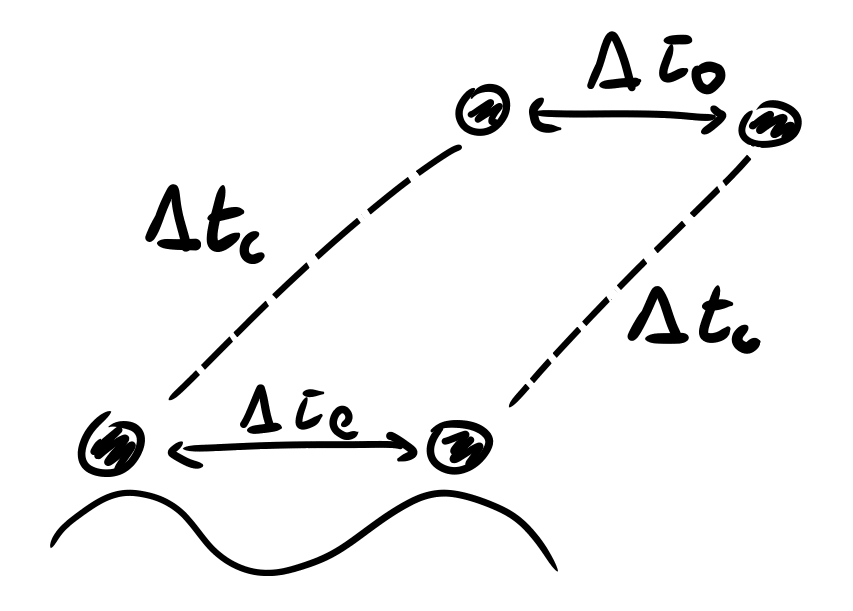
\includegraphics{2018/11/20181109_redshift.png}
    \caption{The setup for our discussion of redshift. An emitter at $r=r_e$ sends out flashes of light at regular intervals of proper time $\Delta \tau_e$, which are received at some coordinate time $\Delta t_c$ later by an observer sitting out at $r=r_o$ and measured at intervals of $\Delta \tau_o$. The emitter and observer agree upon the difference in coordinate time between the flashes, but they (correctly) disagree on the difference in proper time.}
    \label{fig:gravitationalredshift}
\end{figure}

Suppose that $d\theta,d\phi=0$ so that our emitter and observer are only radially separated. Since $ds^2=0$ for null geodesics, the flashes of light from the emitter obey $dt^2=dr^2/V(r)^2$, so the light from a crest takes a coordinate time $\Delta t_c=\int_{r_e}^{r_o}dr/V(r)$ to reach the observer at $r_o$. Since this is the same $\Delta t_c$ for the first and second flash and depends only on $r_e,r_o$, it must be that both the emitter and the observer agree on the coordinate time between flashes, $\Delta t$.

However, for both our emitter sitting at $r_e$ and our observer out at $r_o$, they are both at constant $r$ ($dr=0$) and so $ds^2=-V(r) dt^2$, which means that
\begin{align*}
    \Delta \tau_e^2&=V(r_e)\Delta t^2\\
    \Delta \tau_o^2 &= V(r_o)\Delta t^2.
\end{align*}
That is, our emitter and observer will disagree on the amount of proper time corresponding to the same $\Delta t$ between crests. In particular, since the change in coordinate time $\Delta t$ is the same, it follows that $$\frac{\Delta \tau_e^2}{\Delta \tau_o^2}=\frac{V(r_e)}{V(r_o)}.$$
We find that
\begin{align*}
    \frac{\Delta \tau_e}{\Delta \tau_o}&=\sqrt{\frac{V(r_e)}{V(r_o)}}\\
    &=\sqrt{\frac{1-2M/r_e}{1-2M/r_o}}\\
    &\approx 1-\frac{M}{r_e}+\frac{M}{r_o}\\
    &\approx 1-\frac{M}{r_o r_e}(r_o-r_e),
\end{align*}
so the period of proper time between flashes measured by the observer is slightly greater than the period measured at the emitter. In the weak field limit where $M/r$ is small, $r_o>r_e \implies \Delta \tau_o/\Delta \tau_e > 1$. This is the gravitational redshift, and it was first found by Pound and Rebka in 1959 at Harvard.

But note that if $V(r_0)=0$ then the redshift becomes infinite, which might lead us to think something has gone terribly wrong. However, if $V(r)=0$ then the line element $ds^2$ is not well-defined, so all that's happened is that the coordinates have broken down. 

As it turns out, this is merely a coordinate singularity and not a curvature singularity. One can write down for instance the Riemann tensor and show that nothing bad to the curvature happens at $r\to 2M$, and moreover if we pass to a different set of coordinates, we can pass through the event horizon without issue.

There are many sets of coordinates that have been defined for black holes, but the one we'll introduce today is the Eddington-Finkelstein coordinates. They comprise the following:
\begin{itemize}
    \item Null coordinates: constant along light rays
    \item Retarded coordinates:\footnote{These coordinates seem to be bad at $r=2M$, but in fact they are just what we need to cross the event horizon safely.} $$u=t-r-2M \ln \frac{r-2M}{2M}$$
    \item Advanced coordinates: $$v=t+r+2M\ln \frac{r-2M}{2M}$$
\end{itemize}
Look in particular at the $v,r,\theta,\phi$ coordinates. We have
\begin{align*}
    dv &= dt+(2M\frac{1}{r-2M}+1)dr\\
    &= dt+\frac{r}{r-2m}dr\\
    &= dt+\frac{dr}{V(r)}
\end{align*}
and so the line element becomes
\begin{align*}
    ds^2&= -V(dv -\frac{dr}{V})^2+\frac{dr^2}{V}+r^2(d\theta^2 +\sin^2\theta d\phi^2)\\
    &=-Vdv^2 +2dvdr+r^2(d\theta^2 +\sin^2\theta d\phi^2).
\end{align*}

Our metric now has off diagonal terms, but this is no problem. It is still symmetric if we separate out $dvdr$ and $drdv$, and $\det g =-r^4\sin^2\theta \neq 0$ so we expect it to be invertible. Explicitly we can write it as
$$
g_{ab}=\begin{pmatrix}
    -V & 1 & 0 & 0\\
    1 & 0 & 0 & 0\\
    0&0&r^2&0\\
    0&0&0&r^2\sin^2\theta
\end{pmatrix}.
$$
Moreover the inverse is perfectly well-defined away from $r=0$,\footnote{It might seem like there's also an issue with $\theta=0$, but this is just the regular coordinate badness of spherical polar coordinates. Remember that $\phi$ becomes ill-defined at the north pole, $\theta=0$, even though the north pole is otherwise totally unremarkable as a point on the sphere. This is nothing more than the garden-variety coordinate singularity of generic spherical coordinates.}
$$
g^{ab}=\begin{pmatrix}
    0 & 1 & 0 & 0\\
    1 & V & 0 & 0\\
    0 & 0 & 1/r^2 &0\\
    0 & 0 & 0 & 1/(r^2\sin^2\theta)
\end{pmatrix}.
$$
In particular nothing blows up at $r=2M$, so it seems that we've constructed equally good coordinates to sail past the coordinate singularity at the event horizon.

If we take $v,\theta,\phi$ constant, then $ds^2=0$, so lines of constant $v$ are null lines. ($r$ can of course still change.) One such line has $v=0,r=2M$ (the event horizon itself) and what we discover is that as we pass the event horizon, the light cone has tipped over and any timelike trajectory must be directed towards decreasing $r$. That is, beyond the event horizon ($r<2M$) one can no more escape the gravitational pull of a black hole than one can escape the inexorable march of time(like trajectories).
%insert picture

Curiously, a photon on the surface $V=0$ ($r=2M$) can simply stay there in a stable circular orbit. We call $V=0$ the event horizon, and it is also (by our earlier calculation) a surface of infinite redshift. This is why we call it a black hole-- not only can light not escape, but any light from an infalling emitter will be increasingly redshifted as the emitter approaches the event horizon. If one throws a flashing light clock (i.e. with constant period in its own proper time) into the black hole, an observer sitting far away from the black hole at constant $r$ will see the flashes become increasingly separated, but they will never actually stop.\footnote{It's a bizarre fact that the clock can cross the event horizon in finite time, but due to the redshift, an external observer can never actually see it fall in. Stranger yet is the viewpoint of the infalling observer, who notices nothing unusual with regards to curvature as they pass the event horizon, but looking radially out will see the light from the outside world increasingly blueshifted. As your light cone tips over, you would see the entire future of the universe outside the black hole, but you would never be able to tell anyone what you saw.}

There is a ``hoop conjecture'' widely attributed to Thorne\footnote{Professor Perry mentioned Yau and collaborators contributing to this work, but I was unable to find any sources which substantiated this claim.} which states that if the amount of matter (with a total mass $M$) is confined to a proper distance $l\leq 2M$, then an event horizon will form. The details of this conjecture and attempts to prove it are beyond the scope of this class, so we'll just state it without proof and hope it sounds reasonable.

As a final note for today, there is still one problem with the black hole-- just look at the curvature as a function of $r$. For instance, if we calculate the trace over all components of the Riemann tensor, we see that
$$R_{abcd}R^{abcd}\sim M^2/r^6$$ up to some numerical factors, and as $r\to 0$, $R_{abcd} R^{abcd}\to \infty$ diverges. In electrodynamics we might say that a divergence is simply unphysical because of quantum effects, but there's no sensible theory of quantum gravity that will let us make sense of this yet in a gravitational context. In classical physics we know what to do-- just call the singularity a boundary of spacetime. But it ought to be rather disturbing that one could simply sail not only over the event horizon but over the boundary of spacetime into... where, exactly? This is a major problem for classical (and quantum) gravity and there is no good solution. Yet.\footnote{``That's what I can tell you about singularities. They're there.'' --Malcolm Perry}

\subsection*{Non-lectured aside: cosmic censorship} Here's a little reflection related to Prof. Jorge Santos's essay this year! A priori, point singularities are maybe not so disturbing to us, since they have no spatial extent and you might think a physical observer could never actually cross it. Fair enough. But in spinning (Kerr) and charged (Reissner-Nordstr\"om) black holes, we get entire singular surfaces called Cauchy horizons. Now we could imagine going right through a Cauchy horizon in finite proper time (I haven't proved this, but one can write down the geodesics and show it's true), and beyond the Cauchy horizon, the Einstein equations fail to predict our trajectory based on the past. Determinism breaks down. 

Some physicists (most notably Roger Penrose) have therefore proposed the \term{strong cosmic censorship conjecture}, which suggests (in one phrasing) that Cauchy horizons do not represent physically realizable solutions to the Einstein equations.\footnote{There's also the \term{weak cosmic censorship conjecture} which says roughly that nature always conspires to hide away singularities behind event horizons. The two conjectures are related in spirit but formally distinct.} For instance, it might be that small perturbations (e.g. what are called quasinormal modes) to the event horizon set the black hole ringing like a bell, and this ringing behavior collapses and destroys the Cauchy horizon. Equivalently, if you read my footnote on blueshift earlier (following the discussion of the redshift near the event horizon), you might reason that from the perspective of any infalling observer, all the light from the entire lifetime of the external universe is blueshifted to infinitely high frequency and the energy of this light simply obliterates any poor soul with aspirations of sailing off the edge of spacetime. Cosmic censorship is saved.

Or is it? Recent work by \href{https://news.berkeley.edu/2018/02/20/some-black-holes-erase-your-past/}{Peter Hintz of MIT and others} suggests that there's a loophole in certain kinds of spacetimes. In particular, our solutions assumed asymptotically flat boundary conditions. This is what allows the light from eternity to send our hapless observer to the Shadow Realm. However, if our black hole sits in a positively curved, expanding spacetime (asymptotically de Sitter, not to be confused with anti-de Sitter, AdS), then the blueshift is suppressed by the expansion of spacetime. This is particularly relevant because our universe seems to have a small but non-negligible positive cosmological constant, and therefore looks to be asymptotically de Sitter. Under certain conditions, this suppression is enough to overcome the infinite blowup normally associated with the blueshift. Our observer seems to have gotten a reprieve, at the cost of strong cosmic censorship. Is there another physical argument we've missed which closes this loophole, or is cosmic censorship in real trouble? This is an open research question and the topic of my Part III essay this year.

For additional reading, see Harvey Reall's review \href{https://physics.aps.org/articles/v11/6}{here} as well as the recommended readings for the essay:
\begin{itemize}
    \item V. Cardoso, J. L. Costa, K. Destounis, P. Hintz and A. Jansen, ``Quasinormal modes and Strong Cosmic Censorship,'' Phys. Rev. Lett. \textbf{120}, no. 3, 031103 (2018), \url{https://doi.org/10.1103/PhysRevLett.120.031103}
    \item O. J. C. Dias, H. S. Reall and J. E. Santos, “Strong cosmic censorship: taking the rough with the smooth,” JHEP \textbf{1810}, 001 (2018), \url{https://doi.org/10.1007/JHEP10(2018)001}.
\end{itemize}
